%
% Este archivo es parte de un documento sobre OpenERP/Odoo creado
% y distribuido bajo licencia GNU Free Documen License v1.3.
%
% Para obtener la fuente e información más detallada, visite
% https://github.com/Gabriel-fm/oerp-manual
%
% Copyright (c) 2014 - Gabriel Franco
%

\chapter{Módulo de Contabilidad}

\section{Conceptos previos de Contabilidad}

En este módulo se utilizan lo que se conocen como \textbf{diarios}.

Los \textbf{diarios} no son más que una forma más de agrupar los datos. Las facturas, por ejemplo, pueden guardarse en distintos \emph{diarios}. Esto, al final, no influye en ningún elemento de la factura ni en la gestión de las mismas, siguen siendo las mismas facturas con los mismos datos y los mismos efectos. La diferencia está en que después se puede hacer una busqueda o realizar listados por diarios.

Pueden entenderse estos diarios como carpetas físicas. Las facturas pueden guardarse -- hablando de facturas impresas -- en el mismo lugar y, a la vez, ordenadas en carpetassegún la necesidad, para una mayor organización.

De igual modo, los \textbf{asientos contables} son otro ejemplo de elementos clasificables en diarios. Siguen siendo asientos contables y no se ven alterados por el diario en el que sean almacenados. En este caso se pueden utilizar, por ejemplo, como se ve en la sección \ref{con:asentar}, que puede asentarse todos los asientos de un diario, ahorrando la selección de los mismos.



\section{Clientes}

En la sección de \textbf{clientes} de este módulo se encuentran las distintas opciones en relación a los datos contables sobre los mismos. Desde las facturas a recibos e incluso los mismos datos de clientes y sus fichas.

\subsection{Facturas de clientes}
Esta opción da acceso al área de la aplicación donde se almacenan las facturas realizadas a los clientes (las facturas de ventas). Desde aquí pueden crearse nuevas facturas y ver de un vistazo las ya existentes y algunos de sus datos más importantes.

A pesar de que desde aquí pueden crearse nuevas facturas, hay que recordar que algunas son generadas automáticamente a través de los pedidos de ventas. Los encargados del control y aprobación de facturas deberán estar atentos a las nuevas facturas generadas automáticamente como borrador, que aparecen en azul en el listado, verificando que los datos introducidos son correctos para validar y generar la factura a enviar al cliente.

\begin{figure}[H]
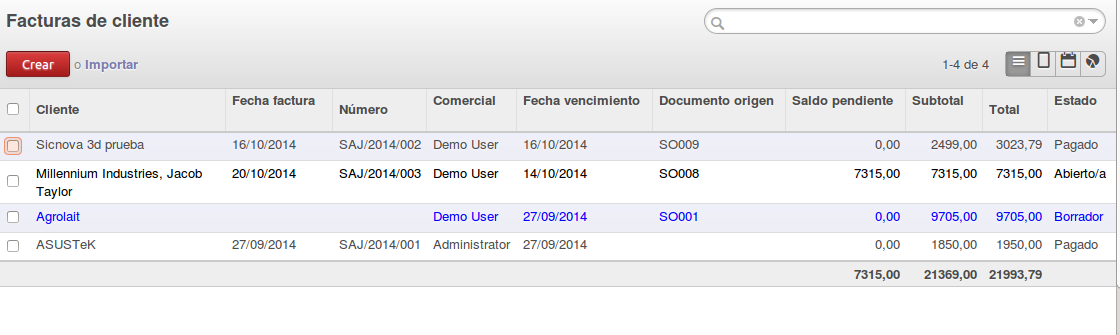
\includegraphics[width=\textwidth]{contabilidad/img/con_lisfact2.png}
\caption{Listado de facturas}
\label{con:lisfact}
\end{figure}


En el listado de facturas (figura \ref{con:lisfact} ) se ven los datos principales de las mismas. El \textbf{Cliente} al que hace referencia la factura, la \textbf{Fecha factura} de cuando fue creada, el \textbf{Número}, que no es más que la numeración de la factura, la cual es además personalizable. 

El \textbf{Comercial} hacereferencia a quién ha gerenardo la factura. Si la factura se crea a mano, este campo será el del usuario
que la ha creado. Si la factura ha sido generada automáticamente a través de una orden de venta, por ejemplo, este campo se rellenará con el nombre del comercial que ha generado dicha orden de venta. De igual manera, el campo \textbf{Documento origen} hará referencia a ese documento (orden de venta, por ejemplo) que ha generado automáticamente la factura.

La \textbf{Fecha de vencimiento} indica, en el caso de utilizar \emph{plazos de pago}. Esta fecha de vencimiento se genera automáticamente de acuerdo a estos plazos. Cuando se utilizan plazos de pagos, se generarán automáticamente los asientos contables en distintas fechas (para por  ejemplo pagos de 50\% en un plazo y el resto en otra fecha, adaptando este campo a estas fechas de asientos. También pueden no utilizarse plazo de pago y forzar una fecha de vencimiento concreta. O no utilizar ni fecha de vencimiento ni plazo de pago, indicando de esta manera que el pago es directo.

El \textbf{Saldo pendiente} indica el dinero pendiente de pago de esa factura. El campo \textbf{Subtotal} muestra el total a facturar \textbf{sin} contar con los impuestos, mientras que en el campo \textbf{Total} si muestra la facturación total incluyendo los impuestos.

El \textbf{Estado} de la factura, cuyos posibles estados son los siguientes:

\begin{itemize}
  \item \textbf{Borrador} -- Estado por defecto para las nuevas facturas. En este punto, las facturas \emph{son todavía editables en todos sus
                             campos}
  \item \textbf{Pro-forma} -- Si el sistema tiene activada la capacidad de generar facturas pro-forma, este estado se encontrará disponible. En
                             este punto, la factura no tiene aún una numeración asignada.
  \item \textbf{Abierto/a} -- En este estado, la factura está confirmada, y se mantiene en este estado hasta que se realiza el pago completo
                             de la misma. Al llegar a este estado, las facturas \emph{no permite editar todos sus campos}, no se pueden cambiar
                             las líneas de factura y otros elementos. Si fuera necesario cambiarlos, habría que \emph{Cancelar} la factura, editarla
                             y volver a aprobarla.
  \item \textbf{Pagada} -- Estado al que se llega automáticamente al introducir el pago (o los pagos) de la factura. Los asientos de estos pagos pueden
                           o no estar conciliados, esto no es relevante para el cambio de estado.
  \item \textbf{Cancelada} -- Estado al cancelar la factura. Las facturas canceladas que ya han sido numeradas (que han pasado por el estado de
                           abierto) \textbf{no pueden ser borradas}, hay que pasarlas a borrador, editarlas con la nueva información
\end{itemize}


\subsubsection{Factura individual}

La figura \ref{con:facindividual} muestra la visión individual de una factura con su pestaña \emph{Líneas de factura} seleccionada. Además de esta pestaña hay otras dos denominadas \emph{Otra información} y \emph{Pagos}

\figura{contabilidad/img/con_facindividual.png}
{Vista individual de edición de una factura}
{con:facindividual}

Al seleccionar en el campo de \textbf{Cliente} uno ya existente, la factura se rellenará automáticamente con los datos de dirección y facturación introducidos en la ficha del cliente, no siendo necesario volver a repetirlos en la factura.

Se debe seleccionar la \textbf{Posición fiscal} si procede y añadirla fecha de la factura si no está completada (si no es una factura creada
automáticamente)

El campo de \textbf{Cuenta} se rellena automáticamente según el cliente, indica en que cuenta se crearán los asientos contables de esta factura  (no incluyendo los impuestos, por supuesto)

En la imágen se puede apreciar también la \textbf{pestaña Líneas de factura}. En esta pestaña se introducen las líneas de facturación, es decir, los productos incluidos en esta factura. Pulsando sobre el texto \emph{Añadir un elemento} se creará una nueva línea en la que se podrá elegir el producto a incluir a través de la columna \emph{Producto}. Al seleccionar el producto se rellenarán automáticamente el resto de campos. Estos se rellenarán con los datos introducidos previamente en el producto, pero pueden ser editados in situ en cada línea, por ejemplo. \textbf{A cada cambio que pueda afectar al precio} se debe, tras el susodicho cambio, pulsar en \emph{(actualizar)}, situado justo encima del calculo total de la cantidad de la factura.

Como \textbf{Plazos de pago} existen algunos por defecto, siendo totalmente configurable según las necesidades de la venta.

De igual forma, el campo de \textbf{Información adicional} se puede utilizar para almacenar cualquier información extra en relación a la factura.


\figura{contabilidad/img/con_pesotra.png}
{Pestaña \emph{Otra información} de una factura}
{con:pesotra}

La figura \ref{con:pesotra} muestra la \textbf{pestaña de \emph{Otra información}}. En la misma se puede observar algunos campos no relacionados de forma totalmente directa con la factura como el \textbf{Comercial} y \textbf{Equipo de ventas} responsables de la factura   el \textbf{Documento origen}-- rellenado automáticamente si la factura se genera automáticamente desde otro documento.

La \textbf{Referencia del cliente} es rellenada automáticamente en el caso de que exista dicha información en la ficha del cliente. De igual forma la \textbf{Cuenta bancaria}, campo que hace referencia al número de cuenta contra el que se pagará la factura, se extrae automáticamente de la ficha del cliente en el caso de que exista tal información con anterioridad. En cualquier otro caso siempre puede rellenarse en este punto.

El \textbf{Periodo contable} puede forzar a la factura a aparecer en determinado periodo contable si se elige alguno aquí. En caso contrario su periodo contable será asignado en función de la fecha de creación.

Los \textbf{Asientos contables}, que se aprecian vacios en la imagen, mostrarán un enlace a estos asientos en el momento en el que la facturasea validada.

Lo último que se puede observar es la \textbf{tabla de impuestos}. En ésta se reflejan los distintos impuestos que se han asignado en las líneas de factura indicando su descripción, la cuenta a la que apuntan los asientos de estos impuestos y la base y el importe del impuesto. Cada impuesto se representa en una línea distina.

\figura{contabilidad/img/con_pesasientos.png}
{Pestaña \emph{Pagos} de la factura}
{con:pesasientos}

La última pestaña es la \textbf{pestaña \emph{Pagos}}. En esta se presenta una tabla que contendrá la información de los pagos realizados para la factura. En esta se aprecia la \textbf{Fecha vigencia} y el \textbf{Asiento contable} asociado a ese pago. También el \textbf{Nombre} y \textbf{Referencia} del pago, información que se rellena cuando se crea este pago.

También aparece el \textbf{Diario} en el que se registra el pago y los campos \textbf{Debe} y \textbf{Haber} que complementan la información sobre el pago indicando la cantidad y dirección de la transacción de dinero.

\subsubsection{Pago de facturas}

La manera más cómoda de registrar los pagos de las facturas es a través de las mismas facturas. Cuando una factura ha sido validada, aparecerá un botón en la zona superior denominado \textbf{Registrar pago} tal como se aprecia en la figura \ref{con:facpagos}. Hacer click en este botón presentará la pantalla de registro de pago que se ve a continuación en la figura \ref{con:facpagar}

\figura{contabilidad/img/con_facpagos.png}
{Botones que aparecen en una factura abierta}
{con:facpagos}

\figura{contabilidad/img/con_facpagar.png}
{Diálogo para el registro de un pago}
{con:facpagar}

La mayoría de datos en el diálogo, se rellenarán de acorde a la información de la factura. El \textbf{Cliente} será el mismo que el indicado en la factura. El \textbf{Importe pagado} se rellenará automáticamente con el saldo pendiente de pago, pero modificable por el usuario. Mediante el \textbf{Método de pago} se indica la forma de pago, a través de banco, con efectivo\ldots

El resto de campos hacen referencia a la \textbf{Fecha} del pago, al \textbf{Periodo} al que pertenece el pago -- por defecto el actual aunque es modificable también por el usuario -- y una \textbf{Ref. Pago}, referencia personalizable del pago  y \textbf{Memoria}, campo también de uso personalizado. Cabe recalcar que estos dos últimos campos son opcionales.

En el momento en el que la suma de los pagos alcance el total de la factura, esta se considerará pagada automáticamente y los asientos serán conciliados.




\subsection{Facturas rectificativas de cliente}

Las \textbf{facturas rectificativas} son, en funcionamiento y en presentación, exactamente iguales que las facturas de cliente vistas en la sección anterior.

Cabe destacar que no es necesario, en la factura rectificativa, añadir cantidades en negativo. Al crear una factura rectificativa se da por sentado que las cantidades no son a cobrar por parte de los clientes, sino a reintegrar a los mismos. Esto quiere decir que una factura rectificativa que incluya, por ejemplo, una impresora, es señal de que se está haciendo una devolución de la misma por parte del cliente al que se le ha vendido -- todo en cifas positivas en la factura.

\subsubsection{Creación de facturas rectificativas}

La creación de facturas rectificativas puede hacerse de dos formas. La primera de ella es a través del botón \textbf{Crear} en la vista del listado de facturas rectificativas de cliente. Con este botón se creará una factura rectificativa vacia, a rellenar por completo por el usuario, incluyendo datos como el cliente, las referencias de la pestaña \emph{Otra información}, las líneas de productos\ldots

Una segunda forma de crear facturas rectificativas es a través del botón \textbf{Reintegrar factura} en las \emph{Facturas de clientes} -- no en las facturas rectificativas -- puede observarse en la figura \ref{con:facpago} de la sección anterior. Aparecerá en las facturas validadas y abiertas y en las pagadas. Con este botón se presentará un diálogo (figura \ref{con:facrect}) en el que se indica como se reintegra la factura y como se rectificará.

\figura{contabilidad/img/con_facrect.png}
{Diálogo de creación de factura rectificativa}
{con:facrect}

Los campos obligatorios son, por un lado, el \textbf{Motivo}, de manera que se indique la razón de la rectificación de la factura, y el \textbf{Método de abono}, que determina como se crea la factura rectificativa. Las opciones de este método de pago y su funcionamiento son:

\begin{itemize}
  \item \textbf{Crear una factura rectificativa borrador} -- Crea una factura rectificativa en el estado de borrador para ser modificada por el
            usuario, pudiendo rectificar líneas de productos
  \item \textbf{Cancelar} -- Esta opción considera que la factura no debería haber sido creada, así pues, crea una factura rectificativa que
            anula aquella que se esté reintegrando, validandola y conciliando la factura de cliente y la rectificativa. La factura 
            rectificativa creada es automáticamente validada, no es posible editarla.
  \item \textbf{Modificar} -- Con la elección de esta opción se indica que se quiere modificar la factura. Como, en teoría, las facturas
            validadas y con una numeración asignada no pueden ser modificadas, esta opción crea una factura rectificativa que cancela -- 
            como la opción anterior -- la factura y las concilia y crea una nueva factura identica a la que se modifica en estado 
            de borrador. 
\end{itemize}






\subsection{Recibo de ventas}

Los recibos de ventas se utilizan para introducir los movimientos contables sin necesidad del uso de una factura. Serían los movimientos generados por un ticket de venta. 

Para estos elementos (puede verse una pantalla de edición en la figura \ref{con:recedita}) los datos mínimos necesarios son:

\begin{itemize}

  \item \textbf{Cuenta} -- Cuenta contable en la que se registrará el pago. Si se elige un cliente y se tiene configurada una cuenta para el
          mismo
  \item \textbf{Pago} -- Hay que indicar la forma de pago
      \begin{itemize}
         \item \textbf{Pagar directamente} -- Se interpreta que el pago ha sido inmediato
         \item \textbf{Pagar tarde o agrupar fondos} -- De esta manera se interpreta que el pago se realizará en una fecha determinada que se puede
              introducir bajo este campo (sólo aparecerá la opción de rellenar una fecha si se elige esta opción)
      \end{itemize}

  \item \textbf{Elementos de la venta} -- Se añaden en la pestaña de \textbf{Información de ventas}. Dentro de éste, hay que completar cuatro
 campos:
      \begin{itemize}
         \item \textbf{Cuenta} -- Cuenta contable referente a la venta (por ejemplo, la 7000000)
         \item \textbf{Descripción} --  Descripción de los productos que se venden.
         \item \textbf{Importe} -- Precio de la compra
         \item \textbf{Impuesto} -- En el caso de aplicar IVA a la compra, habrá que especificarlo en este campo
      \end{itemize}
\end{itemize}



\figura{contabilidad/img/con_recedita.png}
{Edición de un ticket de venta}
{con:recedita}


La creación de tickets de venta conlleva la creación de sus asientos contables correspondientes para ser asentados tras una supervisión de los mismos.




\subsection{Pagos de cliente}

Esta sección se encarga de mostrar -- y crear en caso necesario -- los pagos registrados en las facturas realizados por los clientes.

\figura{contabilidad/img/con_paglista.png}
{Listado de pagos de clientes}
{con:paglista}

De un vistazo se pueden observar los pagos realizados por los clientes, pudiendo determinar la \textbf{Fecha} de realización de los mismos, al igual que el \textbf{Número} que se asigna al pago.

También puede verse la \textbf{Empresa} responsable del pago, la \textbf{Referencia} si se ha introducido alguna, y el \textbf{total} del pago junto a su \textbf{Estado}, el cual puede variar entre estados \emph{Borrador}, \emph{Contabilizado} y \emph{Cancelado}.

\figura{contabilidad/img/con_pagindividual.png}
{Edición de un ticket de venta}
{con:pagindividual}

La información mostrada en una ficha individual de un pago (figura \ref{con:pagindividual} muestra la información sobre el cliente que realiza el pago, y las transacciones realizadas. Estas transacciones especifican el \textbf{Apunte contable} al que pertenece -- visible desde la pestaña \emph{Apuntes contables} de esa misma pantalla --, la \textbf{Cuenta} relacionada con la transacción, las \textbf{Fechas}, tanto de creación como de vencimiento y las diferencias en los \textbf{Saldos} con la transacción.

También puede verse si el asiento se encuentra conciliado al completo o no.


\subsubsection{Creación de pagos}

Desde esta misma sección se pueden crear esos pagos de clientes, no obstante, y debido a la complejidad relativa de esta pantalla, se aconseja -- en la medida de lo posible -- utilizar las funciones de registrar pagos desde las facturas. De esta manera se evitan posibles errores por despistes y asegura que todos los datos creados están relacionados y son consistentes.





\subsection{Clientes}
Los datos que se van a ver aquí son los mismos que se han explicado en la sección \ref{ven:clientes} (Vease esta sección para la explicación de estos datos)

Al seleccionar esta opción del menú, los datos presentados son aquellos clientes que tengan marcado, en la pestaña de ventas y compras de la ficha del mismo, la opción de \emph{Cliente}, situado encima de la otra opción \emph{Proveedor}. Se puede ver dicha opción en la imagen ref{con:fichacliente}

\figura{ventas/img/ven_cliventas.png}
{Ficha del cliente con la pestaña \emph{Ventas y compras}}
{con:fichacliente}











\section{Proveedores}

\subsection{Proveedores}
Los datos que se van a ver aquí son los mismos que se han explicado en la sección \ref{ven:clientes} (Vease esta sección para la explicación de estos datos)

Al seleccionar esta opción del menú, los datos presentados son aquellos clientes que tengan marcado, en la pestaña de ventas y compras de  la ficha del mismo, la opción de \emph{Proveedor}, situado bajo la otra opción \emph{Cliente}. Se puede ver dicha opción en la imagen \ref{con:fichacliente2}

\figura{ventas/img/ven_cliventas.png}
{Ficha del cliente con la pestaña \emph{Ventas y compras}}
{con:fichacliente2}


\subsection{Otras secciones de proveedor}

El resto de secciones en el área de proveedores corresponden a exactamente lo mismo que en el área de clientes, pero con la orientación contraria. 

Esto último quiere decir, obviamente, que las \textbf{Facturas de proveedor} y \textbf{Facturas rectificativas de proveedor} es la información de las facturas realizadas a nuestra empresa por parte de los proveedores. El formato de las mismas para insertarlas aquí es exactamente el mismo que en las facturas que se realizan a los clientes. El software se encargará de que el IVA (por ejemplo, además de otros campos) se dirija a la cuenta adecuada, al IVA de las compras.

Los \textbf{Recibos de compra} son los tickets de compra de distintos elementos (como pueda ser gasolina sin facturar o pequeñas comprar en comercios donde no realicen factura) Se insertan de igual manera que los \emph{Recibos de ventas}

La sección de \textbf{Pagos a proveedores} aglutina las distintas transacciones realizadas hacia los proveedores de igual manera que en \emph{Pagos de cliente} se pueden observar todos los pagos de los clientes hacia nuestra empresa de un solo vistazo.








\section{Banco y caja}
\subsection{Extractos bancarios}
El software permite la introducción y almacenaje de los extractos bancarios. Cuando se edita un extracto se puede ver la pantalla
representada en la figura \ref{con:banextractos}.

Con el \textbf{saldo inicial} introducido, el \textbf{saldo final} es calculado en función de las transacciones introducidas en el 
extracto.

Cabe la posibilidad de insertar cada transacción a mano en las líneas inferiores o bien utilizar el botón \textbf{Importar Facturas}, desde la cual se pueden seleccionar facturas pendientes de cobro o de pago. Con esta acción, se añadirán automáticamente líneas en el extracto con la información de la factura. Por defecto, en el extracto se supone que se paga toda la factura (o lo que queda por pagar de la misma), pero es modificable por el usuario. En el caso de que se realice un pago que complete la factura, se indicará mediante un icono verde a la derecha de la línea, mientras que si no concilia por completo el pago, lo mostrará con un icono rojo.

Cuando el extracto es confirmado, se generarán los asientos a los que hace referencia el extracto, con las cantidades, cuentas y clientes indicados en las lineas del mismo.

\figura{contabilidad/img/con_banextractos.png}
{Extracto bancario}
{con:banextractos}



%\subsection{Registros de caja}







\section{Asientos contables}

\subsection{Apuntes contables}
\figura{contabilidad/img/con_apuapuntes.png}
{Listado de apuntes contables}
{con:apuapuntes}

En la pantalla de apuntes contables se presentará, en forma de listado y filtrado por \textbf{Periodo} y \textbf{Diario} -- como se aprecia en la parte superior izquierda del mismo listado -- todos los apuntes contables (figura \ref{con:apuapuntes})



Desde este mismo punto es posible crear nuevos apuntes contables pulsando sobre el boton \textbf{Crear} y rellenando todos los datos adecuadamente. Hay que tener claro que siempre se ha de situar el mismo valor en el campo \emph{Asiento contable} si lo que se está creando son las partidas y contrapartidas de un asiento ya que sólo se consideran como parte de un mismo asiento, si coinciden en este campo. En caso contrario se entienden como apuntes sueltos, no relacionados con ningún asiento.	



\subsection{Asientos contables}

La opción de \emph{Asientos contables} mostrará todos los asientos, sin filtrar ni por periodo ni por diario como en el caso de los apuntes. La figura \ref{con:apuasientos} muestra la presentación de los mismos.

\figura{contabilidad/img/con_apuasientos.png}
{Listado de asientos contables}
{con:apuasientos}

Los campos que se pueden ver son:

\begin{itemize}
  \item \textbf{Nombre} -- Nombre del apunte
  \item \textbf{Referencia} -- Referencia que puede apuntar a facturas u otros documentos.
  \item \textbf{Fecha} -- Fecha de creación del apunte
  \item \textbf{Periodo} -- Periodo del ejercicio fiscal al que pertenece el apunte.
  \item \textbf{Diario} -- Diario en el que se introduce el apunte.
  \item \textbf{Empresa} -- Empresa cliente (o proveedor) relacionada con esta entrada.
  \item \textbf{Importe} -- Valor total del importe contenido en el apunte.
  \item \textbf{A revisar} -- Permite marcar el asiento en el estado "A revisar" para que un supervisor encargado lo revise dado el caso.
                            No tiene efecto sobre el asiento en ningún aspecto, tan sólo lo etiqueta para su revisión posterior.
  \item \textbf{Estado} -- Estado en el que se encuentra el asiento. En este caso sólo hay dos estados
     \begin{itemize}
       \item No asentado
       \item Asentado
     \end{itemize}
\end{itemize}

Bien utilizando el botón \textbf{Crear} o pulsando sobre uno de los asientos, se puede acceder para ver y editar -- en el caso de que no se encuentre asentado -- cualquier asiento individual. Lo que el usuario verá está presentado en la figura  \ref{con:apuasientoeditar}

\figura{contabilidad/img/con_apuasientoeditar.png}
{Listado de asientos contables}
{con:apuasientoeditar}

El \textbf{Diario} y el \textbf{Periodo} son seleccionables por el usuario y obligatorios. El campo de \textbf{Referencia} es opcional, es autorellenado en caso de que el asiento sea creado automáticamente a partir de una factura o algún otro documento, al igual que los campos de \emph{Diario} y \emph{Periodo}.

En la pestaña de \textbf{Apuntes contables} se pueden ver e introducir los apuntes correspondientes al asiento, los campos a rellenar de los que se dispone son:

\begin{itemize}

  \item \textbf{Nombre} -- El nombre del apunte.
  \item \textbf{Empresa} -- Empresa relacionada con el apunte. No es obligatoria.
  \item \textbf{Cuenta} -- Cuenta a la que hace referencia esa línea de apunte.
  \item \textbf{Fecha de vencimiento} -- Fecha límite para el pago de la línea.
  \item \textbf{Debe -- Haber} -- Campos para introducir la información de Debe y Haber del apunte.
  \item \textbf{Importe divisa} -- En el caso de un asiento multidivisa, aquí debe insertarse el valor de la misma.
  \item \textbf{Cuenta impuesto} -- Cuenta de un impuesto a la que hace referencia el apunte. En este caso hace referencia al código del impuesto, no a la cuenta del mismo (la cual se insertaría en el campo \emph{cuenta}).
  \item \textbf{Importe Impuesto/base} -- Se introduce el valor del monto del impuesto o la base impositiva en función del tipo de cuenta. En el caso de cuentas de tipo impositivo, se utiliza el monto del impuesto. En caso contrario introduce el monto de la base imponible.
  \item \textbf{Estado} -- No es editable por el usuario. Indica si el apunte está cuadrado o no, pudiendo saber si el asiento cuadra finalmente.
  \item \textbf{Conciliar} -- No editable por el usuario. Cuando se realiza la conciliación de los apuntes, se indica en este campo la referencia a la conciliación.
  \item \textbf{Conciliación parcial} -- No editable por el usuario. Igual que en el caso anterior, pero se aplica en el caso de conciliaciones parciales.
\end{itemize}


%\subsection{Diarios de comprobantes}







\section{Planes contables}

Las opciones disponibles  en esta sección se encargan de generar las tablas, en formato legible en pantalla sobre el plan contable actual y sus cuentas y la información sobre impuestos que se encuentra en la contabilidad de la base de datos.

\subsection{Plan contable}

Para la obtención del plan se presenta un diálogo en el que se selecciona tanto el ejercicio fiscal como el rango de \textbf{periodos} entre los que se quiere obtener la información, seleccionando además si para este informe se utilizará la información contenida sólo en los
asientos asentados o la información de todos los asientos -- no asentados incluidos.

El diálogo para la configuración del plan se puede ver en la figura \ref{con:plancontable} y la presentación en pantalla del mismo se puede ver en la figura \ref{con:plancontablefinal}

\figura{contabilidad/img/con_plancontable.png}
{Diálogo para la creación del plan contable}
{con:plancontable}

\figura{contabilidad/img/con_plancontablefinal.png}
{Presentación en pantalla del plan contable}
{con:plancontablefinal}

Si en alguna de las líneas que se ven en el plan contable, se hace click, se abrirá para ver en mayor detalle los asientos correspondientes a esa cuenta seleccionada.

\subsection{Impuestos}

De igual manera que en la sección anterior, al acceder a esta opción se presenta un diálogo para definir que impuestos analizar. La elección en este caso se reduce a un \textbf{periodo} (trimestre, mes...) En caso de que se deje vacio ese campo, el informe se hará  analizando todos los periodos que no esten cerrados.

Otra opción disponible es, al igual que en el informe del plan contable, si para la creación del informe se tendrán en cuenta los asientos asentados o todos, inclusive los que no están asentados (Opción \textbf{Movimientos destino}

En las siguientes figuras se puede ver el diálogo para definir el informe (\ref{con:planimpuestos}) y la presentación en pantalla de la información (\ref{con:planimpuestosfinal})

\figura{contabilidad/img/con_planimpuestos.png}
{Diálogo para la obtención del informe de impuestos}
{con:planimpuestos}

\figura{contabilidad/img/con_planimpuestosfinal.png}
{Presentación en pantalla del informe sobre impuestos}
{con:planimpuestosfinal}

Además, haciendo click sobre alguno de los impuestos, se abrirá en más detalle los movimientos (asientos) relacionados con ese impuesto.


\section{Procesamiento periódico}


\subsection{Asientos Borrador}
\label{con:asentar}
La única opción dentro de esta subsección es \textbf{Asentar asientos}. Como su propio nombre indica, es una utilidad para asentar todos esos asientos que no se encontraran ya en ese estado.

Esta opción abrirá un diálogo (figura \ref{con:aseasientos}) a través del cuál se seleccionará el \textbf{Diario} de asientos que se quiere asentar y el \textbf{periodo}. Tras seleccionar ambos elementos se asentarán todos esos elementos que entren dentro 
de las opciones seleccionadas.

\figura{contabilidad/img/con_aseasientos.png}
{Dialogo de asentamiento de asientos}
{con:aseasientos}



\subsection{Conciliación}

\subsubsection{Conciliación manual}

En esta opción se presentará una lista de todos los movimientos (asientos) no conciliados, organizados por empresas a las que pertenecen estos movimientos. La vista general es la que se observa en la figura \ref{con:conmanual}

\figura{contabilidad/img/con_conmanual.png}
{Pantalla de conciliación manual}
{con:conmanual}

A través de esta pantalla se pueden seleccionar distintos asientos no conciliados y aceptar la conciliación entre ellos. Cuando esta selección y acción se realiza, aparece un diálogo para la confirmación de la conciliación (figura \ref{con:conmanuald1})

\figura{contabilidad/img/con_conmanual_d1.png}
{Diálogo de conciliación manual}
{con:conmanuald1}

Si el importe del desajuste fuese igual a cero, se permitiría realizar una \textbf{Conciliación total}. En el caso de que no lo sea -- como en el ejemplo --, puede realizarse una conciliación parcial o una conciliación con desfase. La \textbf{Conciliación parcial} se utiliza si el cliente va a pagar sólo parte de la factura, dejando conciliados los asientos. Con la \textbf{Conciliación con desfase} crea un movimiento de desajuste para su conciliación a posteriori.

Con la opción de \emph{Conciliación con desfase} se presentará a su vez un diálogo para crear ese Movimiento de desajuste, diálogo que es exactamente igual que la parte inferior del diálogo de conciliación automática (figura \ref{con:conauto}). En este diálogo se completa la información sobre ese movimiento, la cuenta, diario y periodo en el que se creará el desajuste.


\subsubsection{Conciliación automática}
Para que una factura se considere pagada, los apuntes contables de la mismas deben estar conciliados con sus contrapartidas, normalmente pagos. Con esta función de conciliación automática, el programa realiza una búsqueda de apuntes a conciliar en las cuentas en las que se le indica. Encuentra los apuntes, de acorde a las empresas, cuando las cantidades se corresponden realiza la conciliación de esos apuntes. 

La siguiente figura muestra el diálogo de conciliación automática.

\figura{contabilidad/img/con_conauto.png}
{Diálogo de conciliación automática}
{con:conauto}

En el área superior y mediante el botón \textbf{Agregar}, se añaden las cuentas en las que se realizará la busqueda de asientos a conciliar. Como se puede apreciar, muestra información sobre esas cuentas, incluyendo entre otras, información sobre el \textbf{debe} y el \textbf{haber}, mostrando también el \textbf{saldo pendiente}.

El campo \textbf{Fuerza} se refiere al número de importes parciales máximo que pueden agruparse para encontrar una conciliación. Esto quiere decir que, en función de todos los asientos disponibles, los combinará entre ellos (con un máximo de elementos combinados definidos por este campo) para comprobar cuales cuadran para ser conciliados.

Si se selecciona la opción \textbf{Permitir desfase}, creará una entrada en la \emph{cuenta}, \emph{diario} y \emph{periodo} indicados en la parte inferior del diálogo -- la parte bajo el nombre \textbf{Movimiento de desajuste} -- donde también se puede indicar el importe máximo para el que se puede crear esa entrada de desajuste.




\subsection{Asientos recurrentes}

En esta sección se pueden definir y generar asientos que se repitan en el tiempo. Pueden categorizarse aquí elementos como algunos alquileres o gastos que se conocen fijos cada cierto periodo de tiempo.

\subsubsection{Definir asientos recurrentes}

La pantalla a la que se accede a través de ésta sección muestra la lista de asientos que se repiten a lo largo del tiempo. Cada una de estas entradas es accesible de forma individual, pudiendo verse la pantalla como la que se muestra en la figura \ref{con:reclista}.

\figura{contabilidad/img/con_reclista.png}
{Edición de asiento recurrente}
{con:reclista}

En la creación de estos asientos recurrentes es necesario el uso de un \textbf{modelo} (que se puede ver más adelante), usar un \textbf{Nombre} para referenciarse al mismo, e indicarle una \textbf{Fecha inicial}, una \textbf{unidad de tiempo} y un \textbf{ periodo} (cada cuantas unidades de tiempo se repetirá el asiento) además del \textbf{número de periodos}, es decir, el número de repeticiones.

Cuando todas esas opciones se encuentran seleccionadas, se puede hacer uso del botón \textbf{Calcular}. Este botón creará los apuntes (que no los asientos) periódicos y los mostrará en la lista inferior (\emph{Apuntes de asientos periódicos}). El ejemplo anterior mostraría lo que se ve en la figura \ref{con:reclistacal}.

\figura{contabilidad/img/con_reclistacal.png}
{Apuntes de asientos periódicos calculados}
{con:reclistacal}

Sin embargo, se aprecia que los campos \emph{Asiento} no está completado. Con esto, se ha calculado donde estarán los asientos, no los asientos en sí. Para generarlos, debe usarse la siguiente opción en el menú (\emph{Generar asientos}). Una vez generados, se enlazarán en estos campos del listado.

De igual manera, se puede seleccionar, pulsando sobre el apunte en la lista, un asiento ya creado.


\subsubsection{Generar asientos}

Esta opción mostrará el diálogo que se aprecia en la figura \ref{con:recgenerar}. Mediante este, se selecciona una fecha \textbf{hasta la cual} se generarán todos los asientos de los asientos recurrentes que no tengan creados esos asientos. 

Siguiendo el ejemplo anterior, utilizar la fecha a tres meses de la actual, generará tres asientos de alquiler, que además se reflejará en la lista de apuntes del asiento recurrente (el listado visto en la figura \ref{con:reclistacal})

\figura{contabilidad/img/con_recgenerar.png}
{Diálogo de generación de asientos}
{con:recgenerar}


\subsubsection{Modelos}

Los modelos hacen referencia a las entradas del asiento que compondrán cada asiento recurrente. Para el ejemplo del alquiler, se rellenarían los datos tal y como se haría para crear los asientos referidos a un alquiler. Con ello, cada vez que se cree un asiento de este modelo, ese asiento contendrá únicamente esos datos, con las fechas adecuadas en cada caso.


\figura{contabilidad/img/con_recmodelo.png}
{Edición de un model de asiento recurrente}
{con:recmodelo}




\subsection{Fin de periodo}

\subsubsection{Cerrar un periodo}
A través de este elemento, se presentará un listado de los periodos actualmente abiertos (figura \ref{con:finperiodo}). En esta lista se puede seleccionar uno o varios periodos y utilizar el menú desplegable \emph{Más} para seleccionar la opción \textbf{cerrar}.

Otra opción es entrando en la visión individual de periodo, haciendo click sobre el que se desée en la lista, y utilizar el botón \textbf{Cerrar periodo} que aparece en la ficha del mismo.

\figura{contabilidad/img/con_finperiodo.png}
{Listado de periodos a cerrar}
{con:finperiodo}


\subsubsection{Generar asientos de apertura}
Esta opción del menú mostrará un diálogo para generar los asientos de apertura de un ejercicio fiscal en base a los datos del
ejercicio fiscal anterior.

Se ha de indicar el \textbf{ejercicio a cerrar} y el \textbf{ejercicio a abrir}, además de el \textbf{diario} y \textbf{periodo} en 
los que se crearán los asientos de apertura, pudiendo además añadirle un \textbf{Nombre} a esos asientos para poder 
identificarlos apropiadamente.

\figura{contabilidad/img/con_finapertura.png}
{Diálogo de generación de asientos de apertura}
{con:finapertura}



\subsubsection{Cancelar apuntes de cierre}

Esta opción del menú abrirá el diálogo que permite cancelar los apuntes de cierre del año fiscal. Sólo será necesario indicarle
el año fiscal del que hay que cancelar los asientos

\figura{contabilidad/img/con_fincancelar.png}
{Diálogo de cancelación de asientos de cierre}
{con:fincancelar}



\subsubsection{Cerrar un ejercicio fiscal}

Cierra un ejercicio fiscal. El diálogo sólo requerirá de indicarle que ejercicio es el que se debe cerrar.

\figura{contabilidad/img/con_fincierre.png}
{Diálogo de cierre del año fiscal}
{con:fincierre}









\section{Informe}

Este menú permite la generación de distintos informes sobre la contabilidad de la empresa agrupando los datos según los mismos. Genera un archivo PDF en cada ocasión.

Para generar los distintos informes, todos siguen un patrón relativamente fijo al poder filtrar los resultados por fecha, por periodos o por otros parametros como -- por ejemplo en los balances -- aquellas cuentas cuyo total no sea cero.

Cada una de las opciones de informes abrirá una ventana emergente con las distintas opciones para la generación de dichos informes. Generar los informes no modifica ninguna información existente en la base de datos, pudiendo por lo tanto generar todos los que sean necesarios sin temor a modificar nada.

%\subsection{Informes legales}
%\subsubsection{Informes contables}
%\subsubsection{Diarios}

%\subsection{Informes genéricos}
%\subsubsection{Empresas}
%\subsubsection{Impuestos}
